\section{Paths whose image curve is a circle}

\subsection{Unit Circle}

Unit circle is set of points in $\R^2$ defined as $C=\{(x,y)\in\mathbb{R} ^2|x^2+y^2=1\}$. Ellipse is
$C=\{(x,y)\in\mathbb{R} ^2|\frac{x^2}{a^2}+\frac{y^2}{b^2}=1\}$
Has standard parameterization of $\textbf{c}(t)=\big(\cos(t),\sin(t)\big)$.
When parameterizing, always start from $t=0$ reference unless otherwise given.\newline 

\begin{center}
    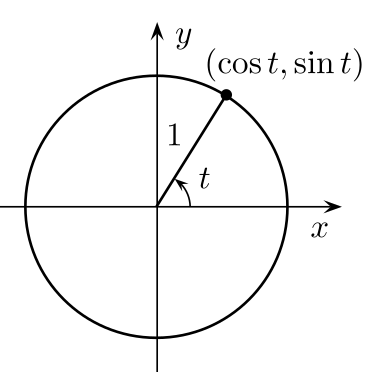
\includegraphics[scale=0.3]{unit-circle.png}
\end{center}

\noindent Properties
\begin{itemize}
    \item Image of $\textbf{c}$ is a closed curve (has no endpoints, plane is divided into $\geq 2$ disjoint regions)
    \item Image of $\textbf{c}$ is a simple curve; no self-intersection 
    \item $\textbf{c}(t)$ is an \textbf{injective path}; path is considered injective if $\textbf{c}(t_1)=\textbf{c}(t_2)$, which implies that $t_1=t_2$ where 
    these are on the open interval $(a,b)$ even if $a=b$
    \item Orientation of $\textbf{c}$ is counter-clockwise in traversal
\end{itemize}

\subsection{Observations}

\[\boxed{\textbf{p}(t)=(a\cos (\pm (nt \pm\theta)) + x_0, b\sin (\pm (nt \pm \theta)) + y_0)}\]

If $-t$ for $t$, orientation is CW, CCW is $t$. If $a=b$, then curve is 
a circle of radius $a$ or $b$, else an ellipse with horizontal and vertical radii.
$x_0$ and $y_0$ simply shift the center coordinate. $n>0\in \R$ determines how many times
the circle is traversed given $t\in[0,2\pi]$, for example. $\theta$ is the phase shift.
When changing direction of traversal, cannot have $a>b$ for $[a,b]$ so to decrease argument of $\sin$ or $\cos$
must have $-t$ for $t$. Starting out, $-t$ goes through the angle range and $t$ is just a sign flip.

\section{Paths whose image is a line or line segment in the plane}

\subsection{Line Parametrics}

A line is a 1D subspace of $\R^2$, so $L=\{t\textbf{m}|t\in\R\}$ for $\textbf{m}\in\R^2$.
$\textbf{m}=\begin{bmatrix}m_x\\m_y\end{bmatrix}$ is the \textbf{slope vector}.
Path given by image of $L$: 

\[\textbf{c}(t)=\left(m_{x} t, m_{y} t\right),t\in\R\]

Can represent $\textbf{c}(t)=t\textbf{m}$ as well.\newline

\noindent
Lines Main Ideas
\begin{itemize}
    \item Image of a line is a curve (e.g. $y=x$ represents image curve of $\textbf{c}(t)=(t,t)$)
    \item Lines can have nonzero intercepts, so $\textbf{c}(t)=t\textbf{m}$ represents $y=2x+1$. Line
    that has intercept vector $P_0=(x_0,y_0)$ $\parallel$ $\textbf{m}=(m_x,m_y)$ can be expressed as:

    \[\boxed{\textbf{c} (t)=(x_0+tm_x, y_0+m_yt)= \textbf{$P_0$}+t \textbf{m} }\]

    Note endpoint of $\textbf{c}(t)$ is on image line (curve).

\end{itemize}

\subsection{General Forms}

2 parametric lines \textbf{collide} if they intersect and the point of intersection corresponds
to the same $t$ in both curves. If you set the parameter vector coordinates equal to each
other and solve for $t$, a solution indicates they collide. Intersection is found by \textbf{eliminating}
the parameter (solve for $t$ in terms of either $x$ or $y$ and plug into the other).\newline

\noindent
General form of parameterized curve can be expressed as the following:

\[\boxed{\textbf{c}(t)=(\frac{m_x}{\Delta t}(t-a)+x_0,\frac{m_y}{\Delta t}(t-a)+y_0)}\]

where $\Delta t$ is the domain interval over $[a,b]$ and $(x_0,y_0)$ represents the desired \textbf{starting coordinate}.
This is important as when going in reverse, other coordinate can be used and slope might be negative.
$a$ is used in $(t-a)$ because everything is conventionally done with respect to starting coordinate.

\section{Paths whose image curve is a line in R3}

\subsection{R3 parameterization}

If $\textbf{m}$ is a nonzero vector along $L$ through origin in $\R^3$, then $L=\{t\textbf{m}|t\in\R\}$;
follows that $\textbf{m}=(m_x,m_y,m_z)$, the slope or direction vector of the line. The basic parameterization is:

\[\textbf{c}(t)=(m_x t,m_y t,m_z t)\]

Basis vectors in $\R^3$ are $\textbf{i}, \textbf{j}, \textbf{k}$. Rewriting parameterization: 

\[\textbf{c}(t)=(x_0+m_x t) \textbf{i}+(y_0+m_y t) \textbf{j}+(z_0+m_z t) \textbf{k}\]

2 lines $\textbf{c}_1(t)=P_0+\textbf{m}_1t$ and $\textbf{c}_2(t)=Q_0+\textbf{m}_2t$ are parallel if
direction vectors are parallel ($\textbf{$m_1$}=k\textbf{m}_2$). Collisions still exist. If neither parallel nor intersecting, considered as skew.\newline

\noindent
To determine skew, parallel, or coincide, use parameters $s,t$ for each line and solve SOE.
If same slope, rule out skew clearly, then check if $s,t\in\R$: if not, then parallel, if so, then they coincide. If intersecting and want to check if collide, some $t$
must satisfy all relations.

\section{Cycloid Problem}

\begin{center}
    \includegraphics*[scale=0.9]{cycloid.png}
\end{center}

With radius 1 and passing through the origin:

\[\textbf{c}(t)=(t-\sin t, 1 - \cos t)\]

Observe that:

\[\textbf{c}^\prime(t)=(1-\cos t, \sin t)\]

Can define the vector $\textbf{u}=\left(\begin{array}{c}x^{\prime}(t) \\0\end{array}\right)$
such that $\textbf{u}$ is always horizontal and $||\textbf{u}||=|x^\prime(t)|$. Reaches maximum
value at $t\in[k\pi|k\in\R]$ and is has minimum cusp where it is 0 at $t\in [2k\pi|k\in\R]$.
Thus, $x^\prime(t)\geq 0$ always, as the x-coordinate is never decreasing. \newline

\noindent
Can also define the vector $\textbf{v}=\left(\begin{array}{c}0 \\y^{\prime}(t)\end{array}\right)$
with the same properties. Reaches maximum value when $t\in[k\frac{\pi}{2}|k\in\R]$.
Can change, as observe $t$ when $\sin t < 0$ or $ >0 $.

\subsection{Hypercycloid Derivation}

\begin{center}
    \includegraphics*[scale=0.5]{Screen Shot 2021-02-06 at 9.40.41 AM.png}
\end{center}

\subsection{Hypocycloid Derivation}

\begin{center}
    \includegraphics*[scale=0.6]{Screen Shot 2021-02-06 at 9.58.04 AM.png}
\end{center}

\section{Velocity Vector}

\subsection{Definitions}

Vector $\textbf{u}(t_0)+\textbf{v}(t_0)$ is he velocity vector to the curve $\textbf{c}(t)$ at $t=t_0$.\newline

\noindent
Let $\textbf{c}:\;[a,b]\rightarrow \R^n$ have a path $\textbf{c}(t)=\left(x_{1}(t), x_{2}(t), x_{3}(t), \ldots, x_{n}(t)\right)$ (let $x_i(t):[a,b]\rightarrow \R$ for each $i$)
\begin{itemize}
    \item If $t_0\in[a,b]$, then $\textbf{c}^{\prime}\left(t_{0}\right):=\left(x_{1}^{\prime}\left(t_{0}\right), x_{2}^{\prime}\left(t_{0}\right), x_{3}^{\prime}\left(t_{0}\right), \ldots, x_{n}^{\prime}\left(t_{0}\right)\right)$; the velocity vector to $\textbf{c}$ at $t_0$
    \item The path $\textbf{c}^{\prime}\left(t_{0}\right):=\left(x_{1}^{\prime}\left(t_{0}\right), x_{2}^{\prime}\left(t_{0}\right), x_{3}^{\prime}\left(t_{0}\right), \ldots, x_{n}^{\prime}\left(t_{0}\right)\right)$; the velocity vector to $\textbf{c}$ is referred to as velocity of $\textbf{c}(t)$
\end{itemize}

Recall chain rule: if $y=f(x)$ where $x$ is a function of $t$, $y\,'(t)=x\,'f\,'(x)$, not to be confused with product rule.
Can write $f\,'(x)=\frac{y\,'(t)}{x\,'(t)}$

\begin{itemize}
    \item If $\textbf{p}(t)=\textbf{c}(t)+\textbf{r}(t),$ then $\textbf{p}^{\prime}(t)=\textbf{c}^{\prime}(t)+\textbf{r}^{\prime}(t)$
    \item If $g(t)=\textbf{c}(t) \cdot \textbf{r}(t),$ then $g^{\prime}(t)=\textbf{c}^{\prime}(t) \cdot \textbf{r}(t)+\textbf{c}(t) \cdot \textbf{r}^{\prime}(t)$
    \item If $\textbf{p}(t)=f(t) \textbf{c}(t),$ then $\textbf{p}^{\prime}(t)=f^{\prime}(t) \textbf{c}(t)+f(t) \textbf{c}^{\prime}(t)$
    \item If $\textbf{p}(t)=\textbf{c}(t) \times \textbf{r}(t),$ then $\textbf{p}^{\prime}(t)=\textbf{c}^{\prime}(t) \times \textbf{r}(t)+\textbf{c}(t) \times \textbf{r}^{\prime}(t)$
    \item If $\textbf{p}(t)=\textbf{c}(f(t)),$ then $\textbf{p}^{\prime}(t)=f^{\prime}(t) \textbf{c}^{\prime}(f(t))$
    \item If $g(t)=\|\textbf{c}(t)\|,$ then $g^{\prime}(t)=\frac{\textbf{c}(t) \cdot \textbf{c}^{\prime}(t)}{\|\textbf{c}(t)\|}$
\end{itemize}

\subsection{Tangent Line}

Tangent line can be visualized as a base vector in standard position plus a velocity vector
tangent to the tip which traces a shifted line in some interval. General formula with base vector $\textbf{c}(t_0)$ and slope $\textbf{c}\,'(t_0)$:

\[\boxed{\ell(t)=\textbf{c}(t_0)+(t-t_0)\textbf{c}\,'(t_0)}\]

\section{Space Curves}

\begin{itemize}
    \item Projection into the $x y$ plane is the path $(x(t), y(t), 0)$.
    \item Projection into the $x z-$ plane is the path $(x(t), 0, z(t))$.
    \item Projection into the $y z$ plane is the path $(0, y(t), z(t))$.
\end{itemize}

\section{Speed and Arclength}

\subsection{Speed}

Speed of a parametric function in $\R^n$ is given by:

$$||\textbf{c}\,'(t)||=\sqrt{\displaystyle\sum_{i=1}^{n}c_i(t)^2}$$

(being the magnitude of the velocity vector)

\subsection{Arclength}

Arclength of a parametric function is given by:

\[S=\int_a^b ||\textbf{c}\,'(t)||dt=\int_a^b\sqrt{(\frac{dx}{dt})^2+(\frac{dy}{dt})^2+(\frac{dz}{dt})^2+\cdots}\;dt\]

Can approximate arclength as a sum of the lengths of secant vector approximations
$\textbf{s}_i=\textbf{c}(t_i)-\textbf{c}(t_{i-1})$:

\[\mbox{arclength}\approx\sum_{i=1}^n||\textbf{s}_i||\]

According to the MVT, there exists a $\hat{t}_i$ in $(t_{i-1},t_i)$ (open interval due to differentiability requirement) such that:

\begin{align*}
    x\,'(\hat{t}_i)&=\frac{x(t_i)-x(t_{i-1})}{t_i-t_{i-1}}\\
    y\,'(\hat{t}_i)&=\frac{y(t_i)-y(t_{i-1})}{t_i-t_{i-1}}
\end{align*}

This means that, since $\textbf{s}_i$ is given as the difference between 2 points,
being a secant:

\begin{align*}
    \textbf{s}_i&=\left((t_i-t_{i-1})x(\hat{t}_i), (t_i-t_{i-1})y(\hat{t}_i)\right )\\
    \textbf{s}_i&=(t_i-t_{i-1})\left(x\,'(\hat{t}_i),y\,'(\hat{t}_i)\right)\\
    \textbf{s}_i&=(t_i-t_{i-1})\textbf{c}\,\,'(\hat{t}_i)
\end{align*}

Thus,

\begin{align*}
    \mbox{arclength}&\approx\sum_{i=1}^n||\textbf{s}_i||\\
    \mbox{arclength}&\approx\sum_{i=1}^n||\Delta t \,\textbf{c}\,\,'(\hat{t}_i)||\\
    \mbox{arclength}&\approx\sum_{i=1}^n\Delta t||\textbf{c}\,\,'(\hat{t}_i)||
\end{align*}

Can define the arclength differential as follows:

\[\mathrm{d}s=\sqrt{\mathrm{d}x^2+\mathrm{d}y^2}\]

Can just define arclength as $\text{arclength}=\int \mathrm{ds}$

\subsection{Arclength Parameterization}

Higher the speed of a curve, farther the points are spaced apart.
An arclength parametrization of a curve is a path whose image is the desired curve and whose speed is constantly one.
Or, $\textbf{c}:[a,b]\to\mathbb{R}^n$ with $||\textbf{c}\,\,'(t)||=1$ for $t\in[a,b]$.
If a curve is not an arclength parameterization, then can do $\frac{\textbf{c}(t)}{||\textbf{c}\,'(t)||}$ but only dividing the coefficients (slopes).\newline

\noindent
When speed is variable, is difficult to define arclength parameterization.
Thus, can define displacement to be $s(t)=\int_a^b (t)dt$. If $v(t)!\neq 0$,
then $s$ is injective because according to FTC, $s\,'(t)=v(t)$.
By definition, $v\,'(t)\geq 0$ always since it is composed of a radical, so it must be \textbf{increasing}.
Thus, if $t_1=t_2$, $s(t_1)\neq s(t_2)$. Arclength parameterization:

\[s(t)=\int_0^t||\textbf{c}\,'(u)||du\]

\noindent
This means that $s$ is invertible, so can solve for $t$ to get $t=\varphi(s)$.
An arclength parameterization can be found by:

\[\boxed{\textbf{p}(s)=\textbf{c}(\varphi(s))}\]

\section{Curvature}

\subsection{Proofs}

Recall that to make an arclength parameterization accumulate the magnitudes of infinitesimal velocity vectors:

\[s(t)=\int_a^t ||\textbf{r}\,'(u)||du\]

Given some curve $\textbf{r}(t)$, define an arclength parameterization by $\textbf{r}(g(s))\rightarrow \textbf{r}_1(s)$, so 
$\textbf{r}$ is defined in terms of $s$. The unit tangent vector $\textbf{T}_1(s)$ is then $\frac{\textbf{r}_1\,'(s)}{||\textbf{r}_1\,'(s)||}=\textbf{r}_1\,'(s)$.

\begin{align*}
    \textbf{T}_1(s)&=\textbf{r}_1\,'(s)\\
    &=\frac{d}{ds}\textbf{r}_1(s)\\
    &=\frac{d}{ds}\textbf{r}(g(s))\\
    &=\textbf{r}\,'(g(s))\cdot g\,'(s)=\textbf{r}\,'(t)\cdot \frac{dt}{ds}\\
    &=\frac{\textbf{r}\,'(t)}{\frac{ds}{dt}}=\frac{\textbf{r}\,'(t)}{||\textbf{r}\,'(t)||}
\end{align*}

This means that $\textbf{T}_1(s)=T(t)$

Continuing, to find curvature $\kappa(t)$:

\begin{align*}
    \textbf{T}_1\,'(s)&=\frac{d}{ds}\textbf{T}(t)\\
    &=\frac{d}{ds}\textbf{T}(g(s))\\
    &=\textbf{T}\,'(t)\cdot \frac{dt}{ds}\\
    &=\frac{\textbf{T}\,'(t)}{\frac{ds}{dt}}\\
    &=\frac{\textbf{T}\,'(t)}{||\textbf{r}\,'(t)||}\\
\end{align*}

Thus, $\boxed{\kappa(t)=\frac{\textbf{T}\,'(t)||}{||\textbf{r}\,'(t)||}}$

\subsection{Definition}

Given a curve $C$ parameterized with arclength by the path $\textbf{c}:[a,b]\rightarrow \R^n$,
curvature is defined as:

\[\boxed{\kappa(s)=||\textbf{T}\,'(s)||}\]

where $\textbf{c}\,'(s)\neq 0$ and $\textbf{T}(s)=\frac{\textbf{c}\,'(s)}{||\textbf{c}\,'(s)||}$ (normalized slope vector).\newline

A loose geometric interpretation is that a greater $\kappa(s)$ implies
more curvature, that is, the curve is changing at a greater rate there.
When $\textbf{c}\,'(s)\neq 0$ is always true for a curve, it is \textbf{regular}.
Is defined in terms of arclength parameterization so curvature
is an intrinsic property of the curve independent of parameterization.\newline

\noindent
Formula for curvature at the point $\textbf{c}(t)$:

\[\boxed{\kappa(t)=\frac{||T\,'(t)||}{||\textbf{c}\,\,'(t)||}=\frac{||\textbf{c}\,\,'(t)\times \textbf{c}\,\,'\,'(t)||}{||\textbf{c}\,\,'(t)||^3}}\]

\section{Motion in 3D space}

Given a path $\textbf{c}: \mathbb{R} \rightarrow \mathbb{R}^{3}$ with $\textbf{c}(t)=(x(t), y(t), z(t)),$ then we have defined:
\begin{itemize}
    \item $\cdot \textbf{v}(t)=\textbf{c}^{\prime}(t)=\left(x^{\prime}(t), y^{\prime}(t), z^{\prime}(t)\right)$ is also path in $\mathbb{R}^{3}$ called the velocity of $\textbf{c}$
    \item $\textbf{a}(t)=\textbf{v}^{\prime}(t)=\textbf{c}^{\prime \prime}(t)=\left(x^{\prime \prime}(t), y^{\prime \prime}(t), z^{\prime \prime}(t)\right)$ is also a path in $\mathbb{R}^{3}$ called the acceleration of $\textbf{c}$
    \item $v(t)=\|\textbf{v}(t)\|=\left\|\textbf{c}^{\prime}(t)\right\|$ is a scalar valued function on $\mathbb{R}$ (that\,'s a fancy way of saying the domain and codomain of this function are both $\mathbb{R}$ ) called the speed of $\textbf{c}$
    \item $\textbf{T}(t)=\frac{\textbf{c}^{\prime}(t)}{v(t)}$ is also a path in $\mathbb{R}^{3}$ called the unit tangent to $\textbf{c}$
    \item $\kappa(t)=\frac{\textbf{T}^{\prime}(t)}{v(t)}=\frac{\left\|\textbf{c}^{\prime}(t) \times \textbf{c}^{\prime \prime}(t)\right\|}{\left\|\textbf{c}^{\prime}(t)\right\|^{3}}$ is a scalar valued function on $\mathbb{R}$ called the curvature of $\textbf{c}$
\end{itemize}

Note that $\textbf{T}\cdot \textbf{T}=||\textbf{v}||^2=1$.
Computing the derivative, $\frac{\mathrm{d}}{\mathrm{d} t} \textbf{T} \cdot \textbf{T}=2 \textbf{T} \cdot \textbf{T}^{\prime}=0$
This means that $\textbf{T}\perp \textbf{T}\,'$.\newline

\noindent
Define $\boxed{\textbf{N}(t)=\frac{\textbf{T}^{\prime}(t)}{\left\|\textbf{T}^{\prime}(t)\right\|}}$ as
the unit normal vector, which is the unit tangent to the unit tangent. From observation, $\textbf{T}\perp \textbf{N}$.
Fact: the acceleration vector always lies in the plane spanned by $\textbf{N}$ and $\textbf{T}$.\newline

\noindent
Acceleration $\textbf{a}(t)$ is thus split component-wise into $a_T$ from $\textbf{T}$
and $a_N$ from $\textbf{N}$:

\[\boxed{a_T=v\,'(t)=\frac{\textbf{a(t)}\cdot \textbf{v}(t)}{v(t)}}\]
\[\boxed{a_N=\kappa(t)v(t)^2=\frac{||\textbf{a}(t)\times \textbf{v}(t)||}{v(t)}=\sqrt{\|\textbf{a}(t)\|^{2}-\left|a_{T}\right|^{2}}}\]

\section{Derivatives of parameterized curves}

\subsection{Arclength parameterization derivation}

Take the following function:

\[\textbf{r}(t)=\langle x(t),y(t) \rangle\]

An arclength parameterization is achieved with the following computation:

\[s=\int_0^t \sqrt{x\,'(u)^2+y\,'(u)^2}\;du\]

Can say that $t=g(s)$, so the arclength parameterization, which is the path in terms of $s$:

\[\textbf{r}_1(s)=\langle x(g(s)),y(g(s))\rangle\]

Taking the derivative by the chain rule:

\begin{align*}
    \textbf{r}_1\,'(s)&=\langle x\,'(g(s))\cdot g\,'(s),y\,'(g(s))\cdot g\,'(s)\rangle \\
    &=g\,'(s)\langle x\,'(t),y\,'(t) \rangle \\
\end{align*}

Note that $g\,'(s)=\frac{dt}{ds}=\frac{1}{\frac{ds}{dt}}=\frac{1}{||\textbf{r}\,'(t)||}$ by taking the derivative of the integral for arclength:

\[\textbf{r}_1\,'(s)=\frac{1}{||\textbf{r}\,'(t)||}\langle x\,'(t),y\,'(t) \rangle=\textbf{T}(t)\]

Following from this, $g\,'(s)=\frac{1}{||\textbf{r}\,'(g(s))||}$ so $g\,'\,'(s)=-\frac{1}{||\textbf{r}\,'(g(s))||^2}\cdot g\,'(s)=-\frac{1}{||\textbf{r}\,'(t)||^3}$

\subsection{Orthogonal derivative and position vectors}

Observe that $\textbf{r}\cdot \textbf{r}=||\textbf{r}||^2$.
Thus, $\frac{d}{dt}[\textbf{r}\cdot \textbf{r}]=2\textbf{r}\cdot\textbf{r}\,'=2||\textbf{r}||||\textbf{r}||\,'$.
Rearranging: $\frac{\textbf{r}\cdot \textbf{r}}{||\textbf{r}||}=||\textbf{r}||\,'$.
Means that magnitude of position vector has to be a constant value in order for it
to be $\perp$ to derivative.

\section{Planetary motion}

\begin{itemize}
    \item Law of ellipses -- orbit of planet is ellipse with sun as focus
    \item Law of equal area in equal time -- position vector pointing from sun to planet sweeps out equal area in equal time (so speed must increase/decrease)
\end{itemize}

Can approximate the area swept in time by $\frac{dA}{dt}=\frac{1}{2}||\textbf{r}(t)\times \textbf{r}\,'(t)||=\frac{1}{2}||\textbf{J}||$.
The differential equation for each of Kepler\,'s laws is: $\textbf{r}\,'\,'(t)=-\frac{k}{||\textbf{r}(t)||^3}\textbf{r}(t)$, so it is in the direction of $\textbf{r}(t)$.
Thus, differentiating $\frac{d\textbf{J}}{dt}=\frac{d}{dt}(\textbf{r}\,'(t)\times \textbf{r}\,'\,'(t))=0$.

\subsection{Cross-product identities}

Cross product identities:
\begin{itemize}
    \item $\boxed{\textbf{u}\times(\textbf{v}\times \textbf{w})=(u\cdot w)\textbf{v}-(\textbf{u}\cdot \textbf{v})\textbf{w}}$
    \item $\boxed{u\cdot(\textbf{v}\times \textbf{w})=v\cdot(\textbf{w}\times \textbf{u})=\textbf{w}\cdot(\textbf{u}\times \textbf{v})}$
\end{itemize}
